% -*- mode:flyspell; mode:latex -*-
\documentclass[12pt]{article}
\addtolength{\oddsidemargin} {-0.885in}
\addtolength{\textwidth}{1.75in}
\addtolength{\evensidemargin}{-0.8in}


\usepackage[latin1]{inputenc}
\usepackage[T1]{fontenc}
\usepackage[english]{babel}
\usepackage{graphicx}
\usepackage{float}
%% \usepackage{siunitx}

%% \usepackage{gensymb}


\usepackage{tikz}
\usepackage{[caption}
\usetikzlibrary{arrows}
\usetikzlibrary{decorations.markings}
\usetikzlibrary{decorations.pathmorphing}
% \usepackage[absolute,overlay]{textpos}
% \usepackage{onimage}

\usepackage{tabularx}
\usepackage{times}
\usepackage{graphics}

% \usepackage{subfigure}
% \usepackage{scalefnt}
%
% \renewcommand\thesubfigure{\arabic{subfigure}}

\usepackage{amsmath}
\usepackage{hyperref}
\usepackage{hhline}
\usepackage{subfig}
\usepackage{color}
\usepackage[all]{hypcap}

\usepackage[normalem]{ulem}  % for striking out
\usepackage{soul}
% \usepackage{fancyhdr}
% \pagestyle{fancy}
% \fancyhead[C]{}
% \fancyhead[L] {\it{Mu2e-doc-29670-v1.0} }
%%%%%%%%%%%%%%%%%%%%%%%%%%%%%%%%%%%%%%%%%%%%%%%%%%%%%%%%%%%%%%%%%%%%%%%%%%%%%%
% use natbib - biblatex not available on Mu2e interactive nodes
%%%%%%%%%%%%%%%%%%%%%%%%%%%%%%%%%%%%%%%%%%%%%%%%%%%%%%%%%%%%%%%%%%%%%%%%%%%%%%
\usepackage[square,sort,comma,numbers]{natbib}

% location of the .bib files: env var BIBINPUTS (~/library/bibliography)

% \usepackage[backend=biber, style=numeric-comp, sorting=ynt] {biblatex}
% \addbibresource{clfv.bib}

% \addbibresource{stntuple.bib}
% \addbibresource{mu2e_web.bib}
% \addbibresource{radiative_pion_capture.bib}

\graphicspath{{figures/}}
%%%%%%%%%%%%%%%%%%%%%%%%%%%%%%%%%%%%%%%%%%%%%%%%%%%%%%%%%%%%%%%%%%%%%%%%%%%%%%
% for portability, make sure all commands are included locally,
%%%%%%%%%%%%%%%%%%%%%%%%%%%%%%%%%%%%%%%%%%%%%%%%%%%%%%%%%%%%%%%%%%%%%%%%%%%%%%
\definecolor{ForestGreen}{RGB}{20,109,20}
%%%%%%%%%%%%%%%%%%%%%%%%%%%%%%%%%%%%%%%%%%%%%%%%%%%%%%%%%%%%%%%%%%%%%%%%%%%%%%%
\newcommand {\abseta}    {\mbox{$\mid \eta \mid $}}
\newcommand {\Au}[1]     {\mbox{$\rm ^{#1}Au$}}          % isotopes of gold

\newcommand {\baftwo}    {\mbox{$BaF_2$}}
\newcommand {\blue}      {\color{blue}}

\newcommand {\deltaE}    {\mbox{$\delta{\rm-electron}$}}

\newcommand {\eemm}      {\mbox{$ee\mu\mu$}}
\newcommand {\emfr}      {\mbox{$\epsilon_{EM}$}}
\newcommand {\eminus}    {\mbox{$e^-$}}
\newcommand {\eplus}     {\mbox{$e^+$}}
\newcommand {\et}        {\mbox{$E_t$}}
\newcommand {\etcorr}    {\mbox{$E_T^{corr}$}}
\newcommand {\etaa}      {\mbox{$\eta$}}

\newcommand {\green}     {\color{ForestGreen}}
\newcommand {\gt}        {\mbox{$>$}}
\newcommand {\gea}       {\mbox{$>=$}}
\newcommand {\gevcsq}    {\mbox{$GeV\!/c^2$}}

\newcommand {\invfb}     {\mbox{$fb^{-1}$}}
\newcommand {\invfbrm}   {\mbox{$\rm fb^{-1}$}}
\newcommand {\invpb}     {\mbox{$pb^{-1}$}}
\newcommand {\invpbrm}   {\mbox{$\rm pb^{-1}$}}
\newcommand {\Ir}[1]     {\mbox{$\rm ^{#1}Ir$}}                 % isotopes of iridium

\newcommand {\jpsi}      {\mbox{$J/\psi$}}

\newcommand {\keVc}      {\mbox{$\rm keV\!/\!c$}}
\newcommand {\kmax}      {\mbox{$k_{\rm max}$}}

\newcommand {\lea}       {\mbox{$<=$}}
\newcommand {\lt}        {\mbox{$<$}}

\newcommand {\mcluster}  {\mbox{$M_{cluster}$}}
\newcommand {\met}       {\mbox{${\not\! E}_{T}$}}
\newcommand {\MeVc}      {\mbox{$\rm MeV\!/c$}}
\newcommand {\MeVcsq}    {\mbox{$\rm MeV\!/c^2$}}
\newcommand {\mmmm}      {\mbox{$\mu\mu\mu\mu$}}
\newcommand {\mt}        {\mbox{$E_{T}$ }}
\newcommand {\mtrkpi}    {\mbox{${M}_{trk+{\pi^0}'s}$ }}

% \newcommand {\mumemconv} {\mbox{$\mu^- A \rightarrow e^- A$}}
% \newcommand {\mumepconv} {\mbox{$\mu^- A \rightarrow e^+ A$}}

\newcommand \mumepconvRelay[1][A]  {\mbox{$\mu^- \textrm{\ArgI} \rightarrow e^+ \textrm{#1}$}}
\newcommand {\MuToEm}     {\mbox{$\mu^- \ra e^-$}}
\newcommand {\MuToEp}     {\mbox{$\mu^- \ra e^+$}}
\newcommand {\MuPToEp}    {\mbox{$\mu^+ \ra e^+$}}

\newcommand {\mumemconv}[1][A] {\mbox{$\mu^- \textrm{#1} \rightarrow e^- \textrm{#1}$}}
% Define a relay to have 2 default arguments instead of limit of 1
\newcommand {\mumepconv}[1][A] {%
  \def\ArgI{{#1}}%store the first argument
  \mumepconvRelay
}

\newcommand {\mzz}       {\mbox{$M_{ZZ}$}}

\newcommand {\pb}        {\mbox{\rm\,pb}}
\newcommand {\Pb}[1]     {\mbox{$\rm ^{#1}Pb$}}           % isotopes of lead: \Pb[208]

\newcommand {\pbar}      {\mbox{$\bar{p}$}}
\newcommand {\pizero}    {\mbox{$\pi^0$}}
\newcommand {\piplusenu} {\mbox{$\pi^+ \to e^+ \nu$}}
\newcommand {\pfake}     {\mbox{$P_{fake}$}}
\newcommand {\ppbar}     {\mbox{$p\bar{p}$}}
\newcommand {\ppbarw}    {\mbox{$p\bar{p} \rightarrow W$}}
\newcommand {\pt}        {\mbox{$P_t$ }}
\newcommand {\purple}    {\color{purple}}

\newcommand {\ra}        {\mbox{$\rightarrow$}}
\newcommand {\red}       {\color{red}}
\newcommand {\Rmue}      {\mbox{$R_{\mu e}$}}

\newcommand {\stat}          {\mbox{\rm (stat.)}}
\newcommand {\statsys}       {\mbox{\rm (stat.+syst.)}}
\newcommand {\syst}          {\mbox{\rm (syst.)}}

\newcommand {\tauenunu}  {\mbox{$\tau \ra e \nu \bar{\nu}$}}
\newcommand {\taumununu} {\mbox{$\tau \ra \mu \nu \bar{\nu}$}}
\newcommand {\tandip}    {\mbox{$\tan \lambda$}}
\newcommand {\ttau}      {\mbox{$\tau$}}
\newcommand {\Tau}       {\mbox{$\tau$}}

\newcommand {\violet}    {\color{violet}}
\newcommand {\vprop}     {\mbox{$v_{prop}$}}

\newcommand {\upar}      {\mbox{$u_{||}$}}
\newcommand {\uperp}     {\mbox{$u_{perp}$}}

\newcommand {\wenu}      {\mbox{$W\rightarrow e\nu$}}
\newcommand {\wlnu}      {\mbox{$W\rightarrow l\nu$}}
\newcommand {\wmunu}     {\mbox{$W\rightarrow \mu \nu$}}
\newcommand {\wpigamma}  {\mbox{$W^{\pm} \rightarrow \pi^{\pm} \gamma$}}
\newcommand {\wtaunu}    {\mbox{$W\rightarrow\tau\nu$}}

\newcommand {\zee}       {\mbox{$Z \rightarrow e^{+}e^{-}$}}
\newcommand {\zll }      {\mbox{$Z       \rightarrow l^{+}l^{-}$}}
\newcommand {\zmumu}     {\mbox{$Z \rightarrow \mu^{+}\mu^{-}$}}
\newcommand {\znunu}     {\mbox{$Z \rightarrow \nu\nu$}}
\newcommand {\zpsigamma} {\mbox{$    Z^{0} \rightarrow J/\psi \gamma$}}
\newcommand {\zpigamma}  {\mbox{$\rm Z^{0} \rightarrow \pi^{0} \gamma$}}
\newcommand {\ztautau}   {\mbox{$Z \rightarrow \tau\tau$}}
\newcommand {\zupsgamma}     {\mbox{$    Z^0 \rightarrow \Upsilon \gamma$}}
\newcommand {\zzx }          {\mbox{$X       \to ZZ$}}
\newcommand {\zzllll}        {\mbox{$ZZ \to \ell^+ \ell^- \ell^+ \ell^-$}}
\newcommand {\zzllnn}        {\mbox{$ZZ \to \ell^+ \ell^- \nu \nu$}}
\newcommand {\zzlljj}        {\mbox{$ZZ \to \ell^+ \ell^- j j$}}
%%%%%%%%%%%%%%%%%%%%%%%%%%%%%%%%%%%%%%%%%%%%%%%%%%%%%%%%%%%%%%%%%%%%%%%%%%%%%%
% editing commands
%%%%%%%%%%%%%%%%%%%%%%%%%%%%%%%%%%%%%%%%%%%%%%%%%%%%%%%%%%%%%%%%%%%%%%%%%%%%%%
\newcommand {\add}[1]    {{\red         {#1}}}
\newcommand {\strike}[1] {{\blue   \sout{#1}}}
\newcommand {\del}[1]    {{\blue   \sout{#1}}}
\newcommand {\dlt}[1]    {{\violet \sout{#1}}}   %alternate delete color
\newcommand {\hlite}[1]  {{\red      \ul{#1}}}   % needs xcolor, soul
%%%%%%%%%%%%%%%%%%%%%%%%%%%%%%%%%%%%%%%%%%%%%%%%%%%%%%%%%%%%%%%%%%%%%%%%%%%%%%%

% %%%%%%%%%%%%%%%%%%%%%%%%%%%%%%%%%%%%%%%%%%%%%%%%%%%%%%%%%%%%%%%%%%%%%%%%%%%%%%
% for editors
% %%%%%%%%%%%%%%%%%%%%%%%%%%%%%%%%%%%%%%%%%%%%%%%%%%%%%%%%%%%%%%%%%%%%%%%%%%%%%%
\newcommand {\pasha}[1]    {{\green  #1}}
\newcommand {\kate}[1]     {{\blue   #1}}
%%%%%%%%%%%%%%%%%%%%%%%%%%%%%%%%%%%%%%%%%%%%%%%%%%%%%%%%%%%%%%%%%%%%%%%%%%%%%%
\begin{document}

\begin{titlepage}
  \begin{flushright}
    \bf {MU2E/PHYSICS/50071} \\
    version 1.02
    \today
 \end{flushright}

  \vspace{1cm}

  \begin{center}
    {\Large \bf MIDAS+ARTDAQ-based data acquisition system for Mu2e
      \vspace{0.3in}
    }

    \vspace{1cm}
    S.Corrodi(ANL), P.Murat(FNAL), ...

    % \footnote{\texttt{Fermilab; e-mail: murat@fnal.gov}}
    \vspace{0.3cm}

    \vspace{0.8cm}
  \end{center}

  \begin{abstract}
    \vspace{0.2in}
    
    We propose a data acquisition system based on MIDAS+ARTDAQ. 
    The system has been tested and 
  \end{abstract}

\end{titlepage}
% \frontmatter
% \chapter*{Abstract}
%
% \addcontentsline{toc}{chapter}{Abstract}
%
% \mainmatter
%
{\tableofcontents}

%%%%%%%%%%%%%%%%%%%%%%%%%%%%%%%%%%%%%%%%%%%%%%%%%%%%%%%%%%%%%%%%%%%%%%%%%%%%%%%
%\chapter{Calibration}
%%%%%%%%%%%%%%%%%%%%%%%%%%%%%%%%%%%%%%%%%%%%%%%%%%%%%%%%%%%%%%%%%%%%%%%%%%%%%%%
% \input{input_data}

%%%%%%%%%%%%%%%%%%%%%%%%%%%%%%%%%%%%%%%%%%%%%%%%%%%%%%%%%%%%%%%%%%%%%%%%%%%%%%%

\newpage
\section {Revision History and TODO items}

\begin{itemize}
\item
  v1.01: version for internal review
\end{itemize}

% {\red
% TODO items:
% 
% \begin{itemize}
% \item
% \end{itemize}
% }
%%%%%%%%%%%%%%%%%%%%%%%%%%%%%%%%%%%%%%%%%%%%%%%%%%%%%%%%%%%%%%%%%%%%%%%%%%%%%%
\newpage
\section {Introduction}
In our view, the Mu2e DAQ in its current form cannot be supported 
by the collaboration during the data taking.
The system is complicated, undocumented, and lacks modularity.
Complexity and lack of the modularity make diagnosing problems
difficult and slow down work of the collaboration.

Although some progress has been made, after years of trying,
no Mu2e collaborator can currently operate the system in their own. 
With a few months left before the start of the cosmic run,
the system has missing pieces yet to be designed. 

We have developed and prototyped a DAQ system based on ARTDAQ and MIDAS.

ARTDAQ is a software for a trigger farm developed at Fermilab and used
by several neutrino experiments. 

MIDAS is a full DAQ suite
\begin{itemize}
\item 
  is used by multiple running and future muon experiments, 
  including g-2, MEG-II, and Mu3e at PSI.
\item
  Is architecture had been tuned and debugged by decades of experience.
  New collaborators joining Mu2e will likely know MIDAS.
\end{itemize}

MIDAQ + ARTDAQ combination will provide a solid and reliable foundation
of the Mu2e DAQ.

\section{System architecture}

The proposed system consists of two big software components :
\begin{itemize}
\item
  ARTDAQ : handles the trigger farm and the data processing
\item
  MIDAS : handles the run configuration, run control, messaging,
  standardizes interfaces between various parts of the online system,
  and provides web-based interface for the shifters,
\end{itemize}

The DAQ architecture is schematically presented in Figure ~\ref{figure:system_architecture}
\begin{figure}[H]
  \begin{tikzpicture}
    \node[anchor=south west,inner sep=0] at (0,0.) {
      % \node[shift={(0 cm,0.cm)},inner sep=0,rotate={90}] at (0,0) {}
      \makebox[\textwidth][c] {
        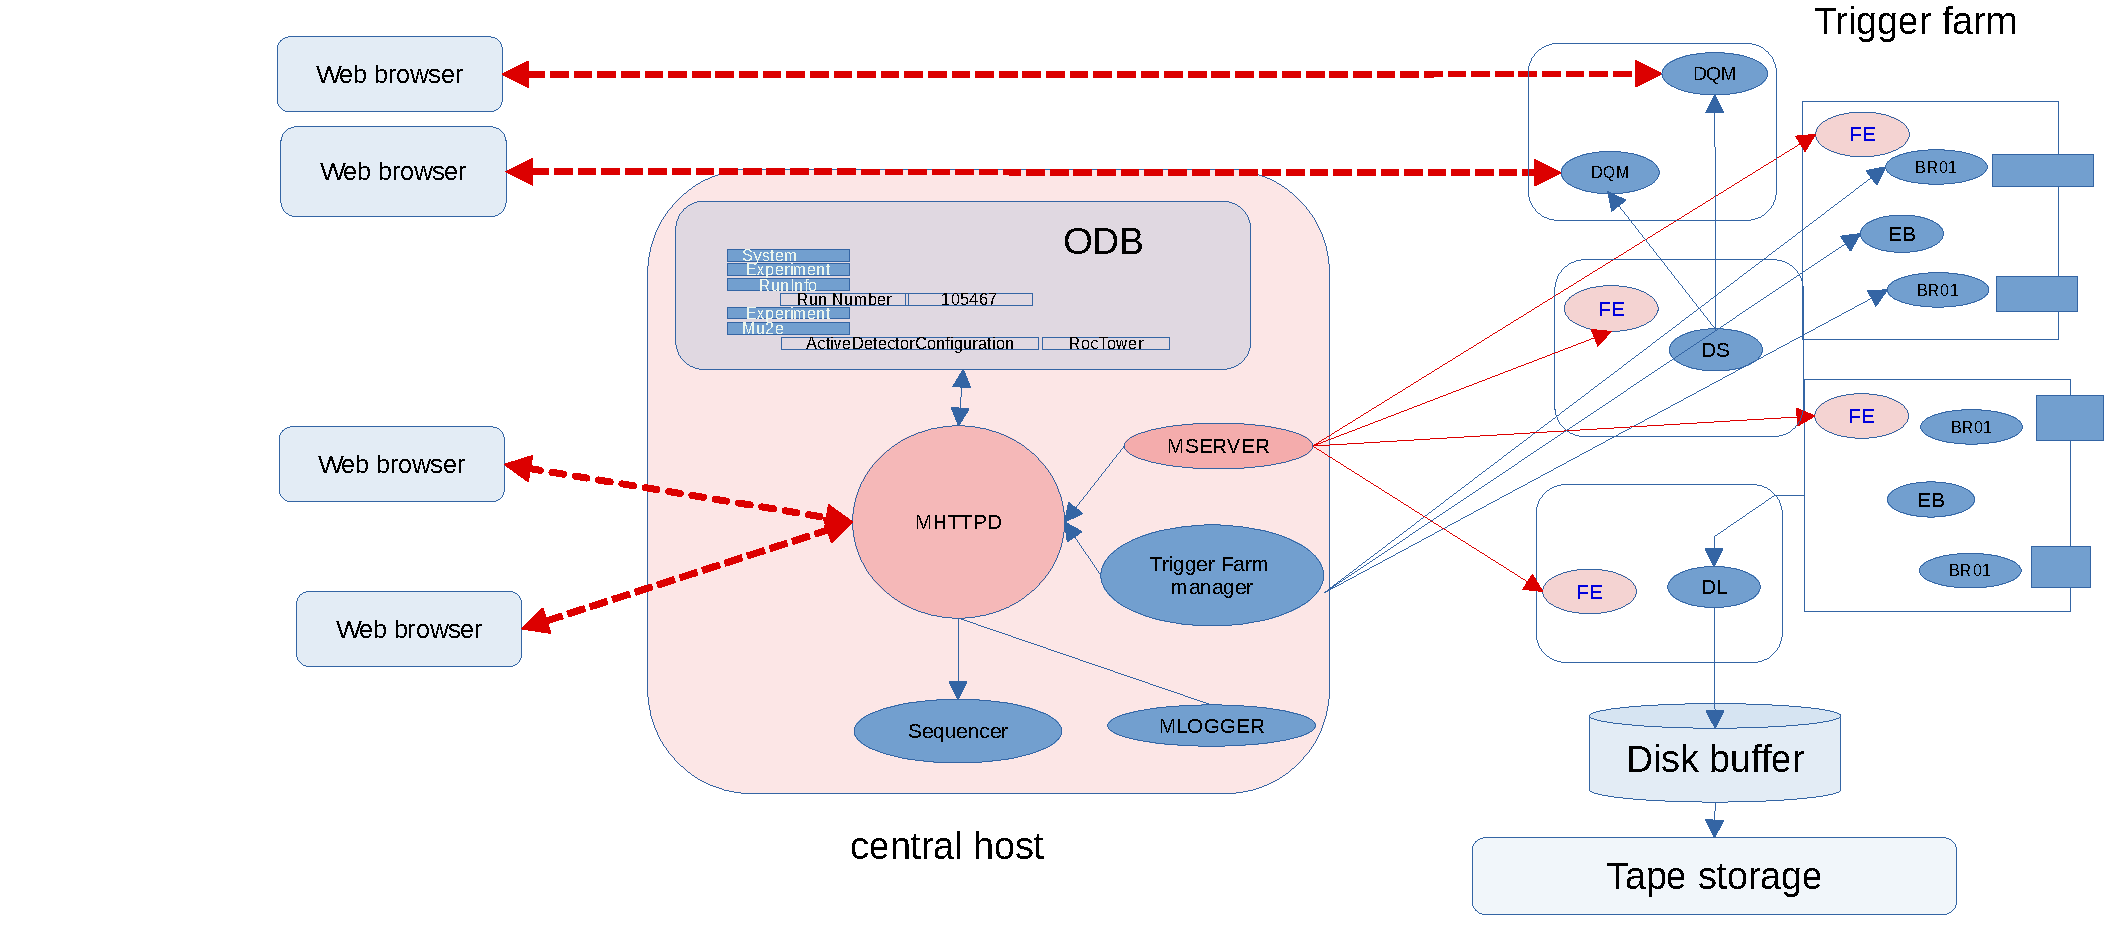
\includegraphics[width=1.1\textwidth]{pdf/system_architecture}
      }
    };
    % \node [text width=8cm, scale=1.0] at (14.5,0.5) {$\mu_B$, expected background mean};
    % \node [text width=8cm, scale=1.0, rotate={90}] at (1.5,7.5) { $S_{D}$, ``discovery'' signal strength  };
  \end{tikzpicture}
  \caption{
    \label{figure:system_architecture}
    Architecture of the MIDAS-based DAQ system
  }
\end{figure}

%%%%%%%%%%%%%%%%%%%%%%%%%%%%%%%%%%%%%%%%%%%%%%%%%%%%%%%%%%%%%%%%%%%%%%%%%%%%%%
\subsection{MIDAS}

COre parts of MIDAS are :

\begin{itemize}
\item 
  mhttpd, a web server with restricted functionality
  mhttpd connects its clients to ODB. 
  The mhttpd doesn't execute any applications. Instead, it only updates the ODB.
\item
  Clients: frontends, communicating with the hardware and other
  parts of the system. Different types of frontends. Mu2e only needs slow monitoring.
\item
  Online DataBase (ODB) - a shared memory segment, which stores all configuration data of the system. Despite its name, ODB is not a database. Instead, it stores only current configuration
  of the system, As the new run starts, a run number-stamped configuration is exported and stored.
  Logical organization of ODB maps onto a json structure and is well suited for describing
  complex configurations with multiple levels of hierarchy
\end{itemize}

MIDAS ODB has several interfaces:
\begin{itemize}
\item 
  web-based interface - via the mhttpd ODB page
\item
  command line interface (odbedit)
\item
  C++ interface allowing C++ clients to interact with ODB
\item
  python interface
\end{itemize}

In all cases, clients connect to MHTTPD and MHTTPD acts as
the only agent directly interacting with the ODB.

%%%%%%%%%%%%%%%%%%%%%%%%%%%%%%%%%%%%%%%%%%%%%%%%%%%%%%%%%%%%%%%%%%%%%%%%%%%%%%
\subsection{Frontends}

MIDAS supports frontends of different types, which include the data readout and monitoring
frontends.

MIDAS event building functionality is not used , done by ARTDAQ.

The architecture of the Mu2e DAQ requires only monitoring and slow control frontends.


%%%%%%%%%%%%%%%%%%%%%%%%%%%%%%%%%%%%%%%%%%%%%%%%%%%%%%%%%%%%%%%%%%%%%%%%%%%%%%
\subsection{Interface to ARTDAQ}
All high bandwidth traffic goes through ARTDAQ.

ARTDAQ processes are controlled by the Trigger Farm Manager (TFM) frontend,
tfm\_launch\_fe.py.

\begin{itemize}
\item 
  TFM reads its initial settings from the "/Mu2e/ActiveRunConfiguration/DAQ/Tfm"
  ODB configuration path.
\item
  FCL files of ARTDAQ processes are stored in \$MU2E\_DAQ\_DIR/config/\$run\_configuration
  subdirectory assumed to be the same (network mounted) on all DAQ nodes.
  The FCL files could be regenerated manually based on the run configuration and the trigger table.
\item
  Archival mechanism: the FCL files used for a given run are stored
  in \$DAQ\_OUTPUT\_TOP/run\_records/\$run\_number area of the node where the TFM frontend is running.
\item
  the log files of ARTDAQ processes running on a given node are stored in \$DAQ\_OUTPUT\_TOP/logs
  directory of that node
\end{itemize}

%%%%%%%%%%%%%%%%%%%%%%%%%%%%%%%%%%%%%%%%%%%%%%%%%%%%%%%%%%%%%%%%%%%%%%%%%%%%%%
\subsubsection{Naming conventions for ARTDAQ components}

It is assumed that :
\begin{itemize}
\item 
  artdaq boardreaders described in the configuration have names "br01", "br02", etc
\item 
  artdaq event builders have names "eb01", "eb02", etc
\item 
  artdaq data loggers have names "dl01", "dl02", etc
\item 
  artdaq dispatchers have names "ds01", "ds02", etc
\end{itemize}

This convention allows to use component names, as they are, in the monitoring system.

%%%%%%%%%%%%%%%%%%%%%%%%%%%%%%%%%%%%%%%%%%%%%%%%%%%%%%%%%%%%%%%%%%%%%%%%%%%%%%
\subsubsection{Port assignment for ARTDAQ XML-RPC communication}
\begin{itemize}
\item
  base\_port: 10000+1000*partition\_number
\item 
  TFM : base\_port
\item 
  MIDAS node monitoring frontend: base\_port+11;
\item 
  artdaq boardreaders: base\_port+101 and base\_port+102
\item 
  artdaq event builders : base\_port + 201 - base\_port+300;
\item 
  artdaq data loggers  : base\_port + 301 - base\_port+400;
\item 
  artdaq dispatchers : base\_port + 401 - base\_port+500
\end{itemize}


%%%%%%%%%%%%%%%%%%%%%%%%%%%%%%%%%%%%%%%%%%%%%%%%%%%%%%%%%%%%%%%%%%%%%%%%%%%
\subsubsection{Communication with ARTRAQ}

\begin{itemize}
\item
  native artdaq communication is internal to the ARTDAQ
\item
  ARTDAQ processes report their metrics in XML-RPC format,
  and it is assumed that parsing of the metrics, visualizing
  it and generating alarms is the job of the 3-rd party application,
  i.e. {\bf grafana}.
\item
  TFM queries the ARTDAQ process metrics over XML-RPC and records
  them in ODB. That obsoletes the need in the 3rd party applications.
\item
  Mu2e -specific applications, i.e. the boardreaders and the filter modules 
  communicate to the MIDAS server directly via messaging and report 
  their status. Therefore simple alarms like single ROC timeouts etc
  could be generated as they are detected. 
  This avoids a need in an additional software to recognize an alarming
  situation and trigger the corresponding notification mechanism.
\end{itemize}


%%%%%%%%%%%%%%%%%%%%%%%%%%%%%%%%%%%%%%%%%%%%%%%%%%%%%%%%%%%%%%%%%%%%%%%%%%%%%%
\subsection{Interface to the online run conditions database} 

\begin{itemize}
\item
  the interface is provided by the MIDAS Sequencer and 
  \href{https://github.com/pavel1murat/frontends/blob/main/conf/mu2e_config_fe.py}
  {\blue the global configuration frontend}.
\item
  before the TFM starts, the configuration frontend requests a new run 
  number from the run configuration DB.
\item
  at begin run, the TFM frontend passes the run number to ARTDAQ processes.
\item
  the global configuration frontend registers the start and the stop of each
  run transition in the run configuration database.
\end{itemize}


%%%%%%%%%%%%%%%%%%%%%%%%%%%%%%%%%%%%%%%%%%%%%%%%%%%%%%%%%%%%%%%%%%%%%%%%%%%%%% 
\subsection{Slow monitoring}

MIDAS history system provides the framework for slow monitoring.
The historical data could be stored in  MIDAS internal format or in a database.
The list of supported databases includes ODBC, SQLITE, MYSQL and PGSQL.

This functionality is similar to that of grafana, however integrated with the
rest of the system

\begin{itemize}
\item
  one monitoring frontend per node 
  \begin{itemize}
  \item
    controls and configures DTC's and ROCs on this node
  \item
    controls the CFO if the CFO is running on this node
  \item
    monitors DTCs and ROCs, collecting history and non-history information
  \item
    monitors artdaq processes d separate collection of the monitoring information and its visualization
  \end{itemize}
\end{itemize}

Figure ~\ref{figure:slow_controls_node_page} gives an example of one of the slow controls pages

\begin{figure}[H]
  \begin{tikzpicture}
    \node[anchor=south west,inner sep=0] at (0,0.) {
      % \node[shift={(0 cm,0.cm)},inner sep=0,rotate={90}] at (0,0) {}
      \makebox[\textwidth][c] {
        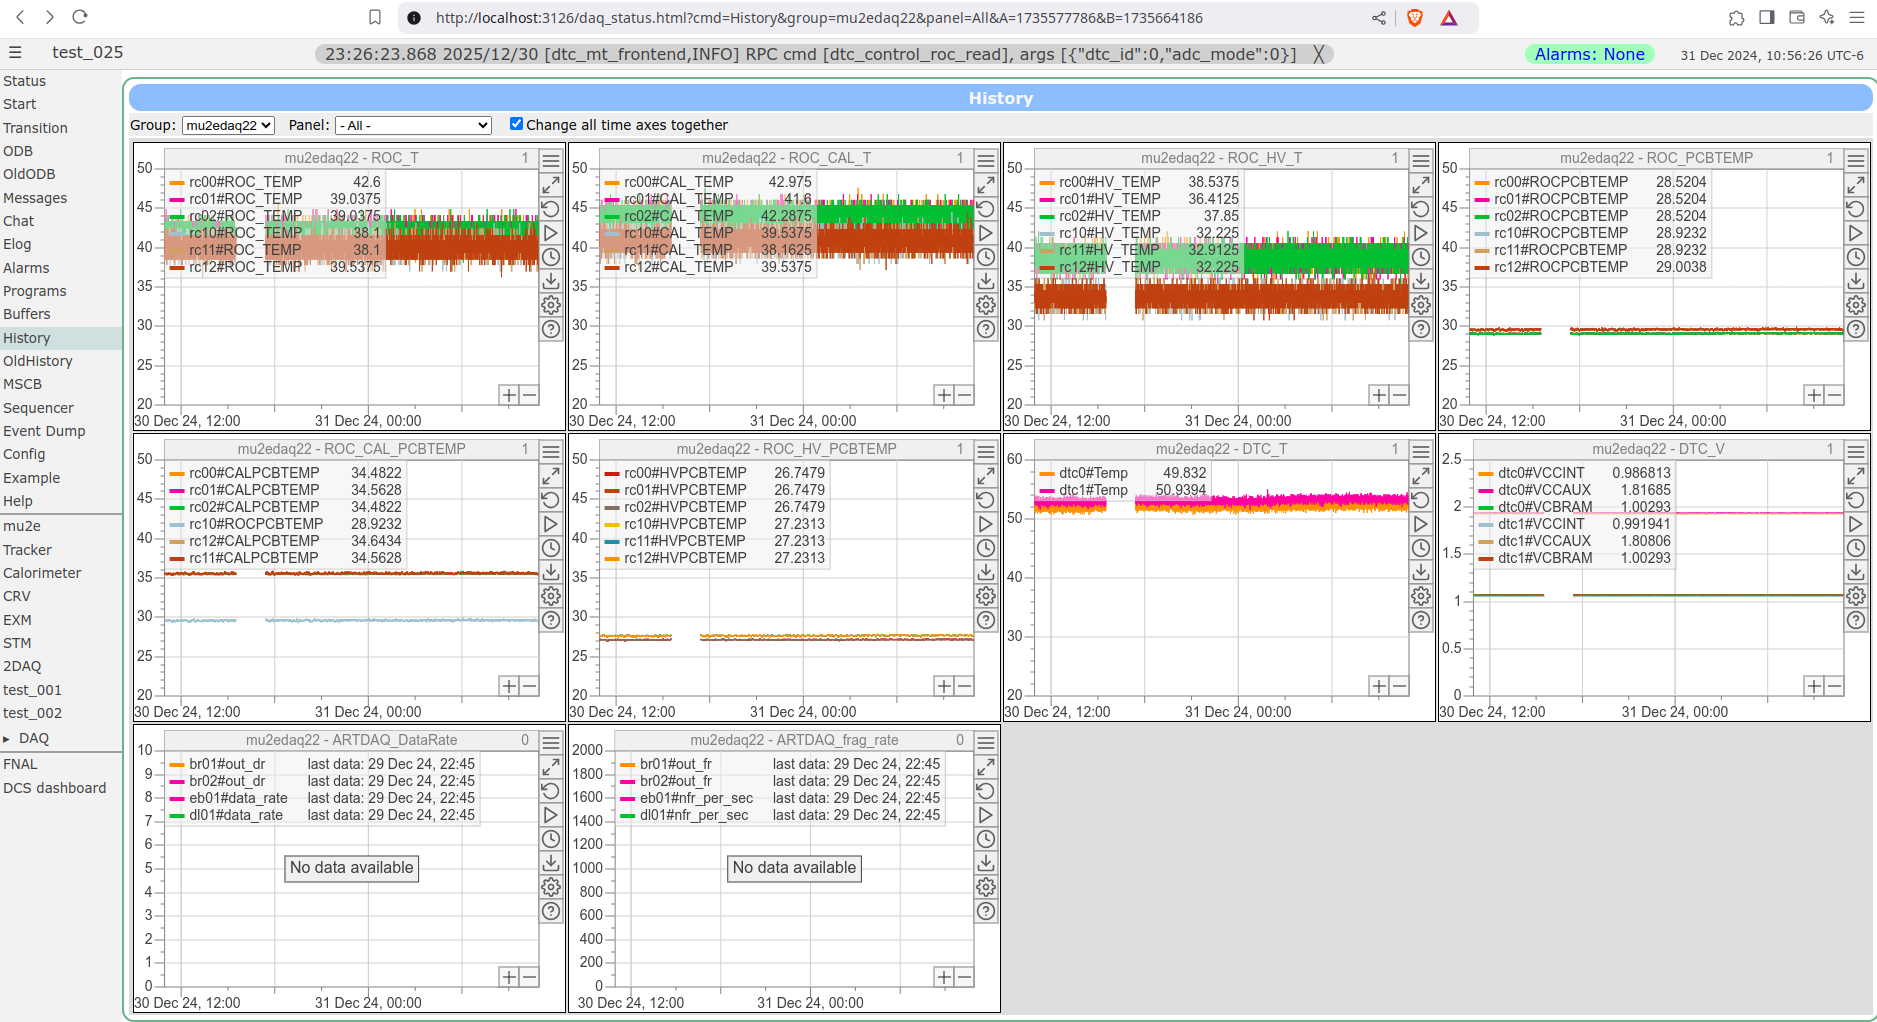
\includegraphics[width=0.95\textwidth]{png/slow_controls_node_page}
      }
    };
    % \node [text width=8cm, scale=1.0] at (14.5,0.5) {$\mu_B$, expected background mean};
    % \node [text width=8cm, scale=1.0, rotate={90}] at (1.5,7.5) { $S_{D}$, ``discovery'' signal strength  };
  \end{tikzpicture}
  \caption{
    \label{figure:slow_controls_node_page}
    A prototype of the DAQ node slow control page. Monitored are the DTC and ROC temperatures and voltages
    and rates of the ARTDAQ processes
  }
\end{figure}


%%%%%%%%%%%%%%%%%%%%%%%%%%%%%%%%%%%%%%%%%%%%%%%%%%%%%%%%%%%%%%%%%%%%%%%%%%%%%%
\subsection{Alarm system}

MIDAS has a built-in alarm system which could be used to inform shifters
about various categories of failures.

That is not a replacement for critical alarms coming from different inputs.
CRYO ? Accelerator ? -{\red talk to Andy Hocker.}


%%%%%%%%%%%%%%%%%%%%%%%%%%%%%%%%%%%%%%%%%%%%%%%%%%%%%%%%%%%%%%%%%%%%%%%%%%%%%% 
\subsection{Javascript web interface}

\begin{itemize}
\item 
  MIDAS web interface is a combination of HTML5+Javascript, based on the
  asynchronous approach to the web pages update (Ajax).
\item 
  MIDAS provides Javascript API to ODB, which facilitates development of
  functional experiment-specific {\bf custom} web pages.
  The interface is documented at \\
  \href{https://daq00.triumf.ca/MidasWiki/index.php/Custom\_Page}
  {\blue https://daq00.triumf.ca/MidasWiki/index.php/Custom\_Page}
\end{itemize}


%%%%%%%%%%%%%%%%%%%%%%%%%%%%%%%%%%%%%%%%%%%%%%%%%%%%%%%%%%%%%%%%%%%%%%%%%%%%%%
\subsection{Interfaces to ECL, ELOG, Slack}

MIDAS has interfaces to internal and external ELOGs and Slack.
\begin{itemize}
\item
  interface to the external ELOG has been implemented and tested
\item
  interface to Slack has been tested and used by at least two experiments - MEG and g-2
\item
  interface to ECL - to be implemented
\end{itemize}


%%%%%%%%%%%%%%%%%%%%%%%%%%%%%%%%%%%%%%%%%%%%%%%%%%%%%%%%%%%%%%%%%%%%%%%%%%%%%%
\subsection{Interface to EPICS}

Although MIDAS has its own history system , it also has an interface to EPICS,
implemented as a slow control frontend

%%% Local Variables:
%%% mode: latex
%%% TeX-master: t
%%% End:


%%%%%%%%%%%%%%%%%%%%%%%%%%%%%%%%%%%%%%%%%%%%%%%%%%%%%%%%%%%%%%%%%%%%%%%%%%%%%%
\subsection{DQM}

DQM processes use ROOT-based histogramming. As any ROOT executable is a web server,
the DAQM jobs publish their histograms on the web, and their clients (users)
simply connect to them over the http protocol.

%%%%%%%%%%%%%%%%%%%%%%%%%%%%%%%%%%%%%%%%%%%%%%%%%%%%%%%%%%%%%%%%%%%%%%%%%%%%%% 
\subsection{Interprocess communication} 

The system supports three mechanisms
\begin{itemize}
\item
  via ODB : some clients write into ODB, others read
\item
  separate collection of the monitoring information and its visualization
\item
  MIDAS messaging: jsonrpc.
  \begin{itemize}
  \item
    Each client can have a jsonrpc server and receive messages
    from any other client.
  \item
    clients can broadcast messages to the system (info and alarm)
    and communicate to each other
  \item
    each frontend, C++ or Python, has a built-in jsonrpc communication
    functionality built-in.
  \end{itemize}
\item
  communication between ARTDAQ processes is based on an older technology,
  XML-RPC. The TFM frontend supports the XML-RPC-based ARTDAQ communication
  protocol.
\end{itemize}

%%%%%%%%%%%%%%%%%%%%%%%%%%%%%%%%%%%%%%%%%%%%%%%%%%%%%%%%%%%%%%%%%%%%%%%%%%%%%%
\section{Configuring the Mu2e DAQ }

The system supports multiple configurations, as shown in Figure~\ref{figure:run_configurations}

\begin{itemize}
\item 
  The configurations are stored in "/Mu2e/RunConfigurations" subtree
\item
  each configuration is an independent subtree, any modification of a given 
  configuration doesn't affect other configurations
\item
  a configuration can be saved as a .json structure and loaded from an external .json file
\item
  ODB links are allowed, but have to point within the configuration
\end{itemize}

\begin{figure}[H]
  \begin{tikzpicture}
    \node[anchor=south west,inner sep=0] at (0,0.) {
      % \node[shift={(0 cm,0.cm)},inner sep=0,rotate={90}] at (0,0) {}
      \makebox[\textwidth][c] {
        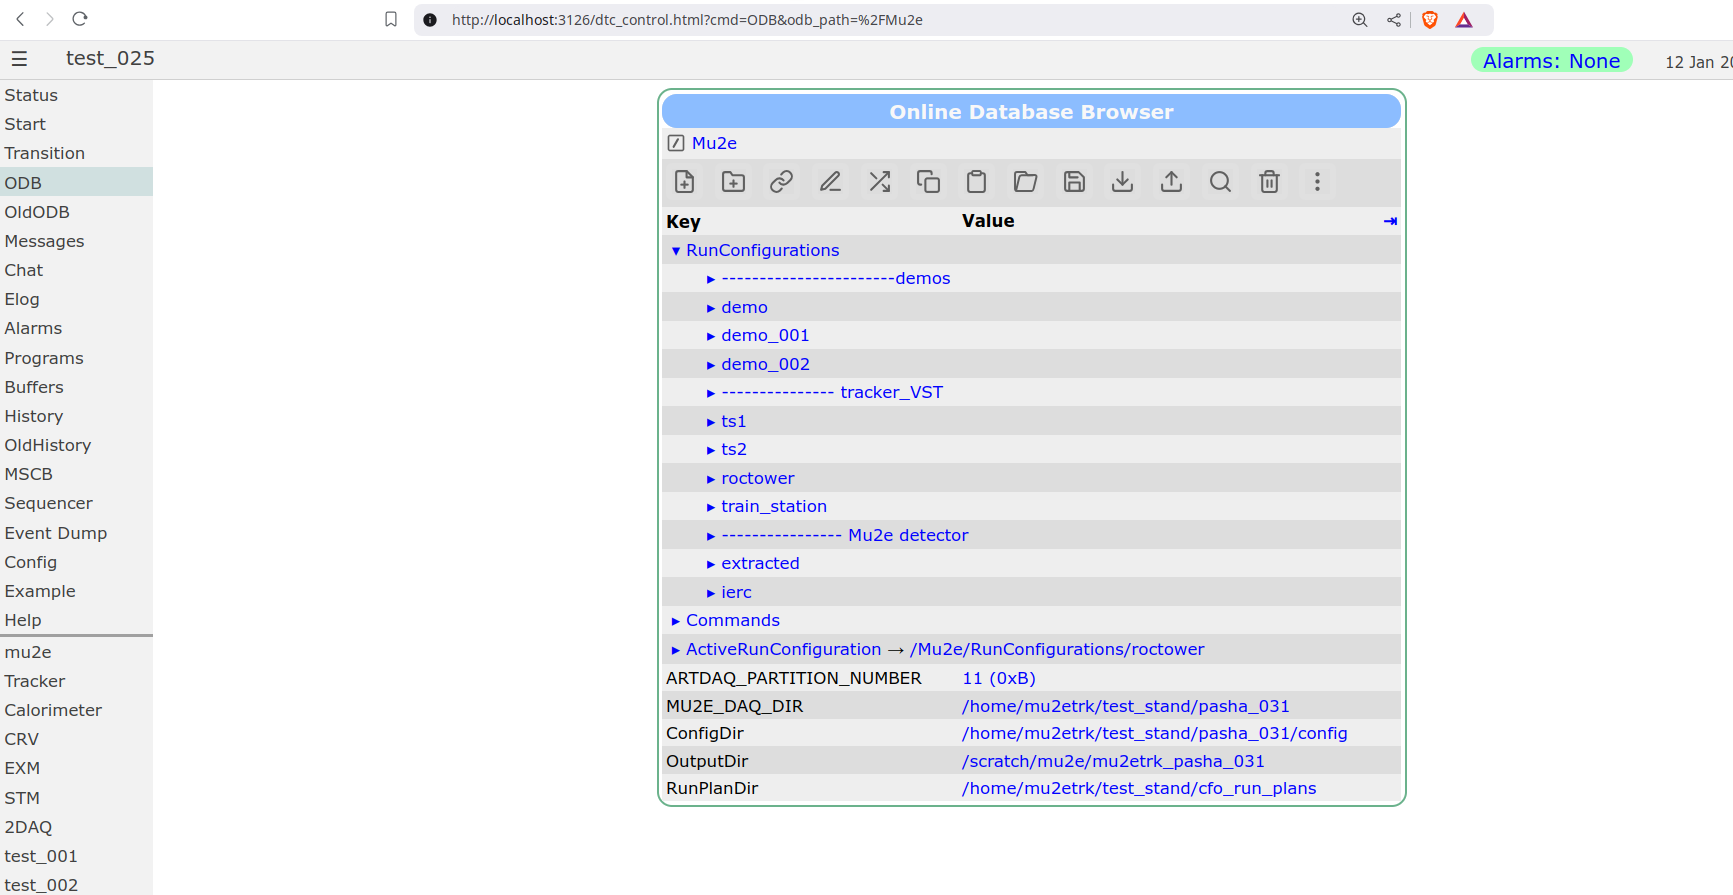
\includegraphics[width=0.95\textwidth]{png/run_configurations}
      }
    };
    % \node [text width=8cm, scale=1.0] at (14.5,0.5) {$\mu_B$, expected background mean};
    % \node [text width=8cm, scale=1.0, rotate={90}] at (1.5,7.5) { $S_{D}$, ``discovery'' signal strength  };
  \end{tikzpicture}
  \caption{
    \label{figure:run_configurations}
    Top-level run configurations
  }
\end{figure}

\begin{itemize}
\item 
  a configuration has a name, a status, and a list of subdetector configurations,
  as shown in Figure~\ref{figure:configuration_top}
\item
  each subdetector has a separate configuration subtree
\item
  templates for the subdetector configurations are stored in the 
  \href{https://github.com/pavel1murat/frontends/tree/main/odb/Mu2e/Subdetectors}
  {\blue frontends/odb/Mu2e/Subdetectors} subdirectory
\end{itemize}

\begin{figure}[H]
  \begin{tikzpicture}
    \node[anchor=south west,inner sep=0] at (0,0.) {
      % \node[shift={(0 cm,0.cm)},inner sep=0,rotate={90}] at (0,0) {}
      \makebox[\textwidth][c] {
        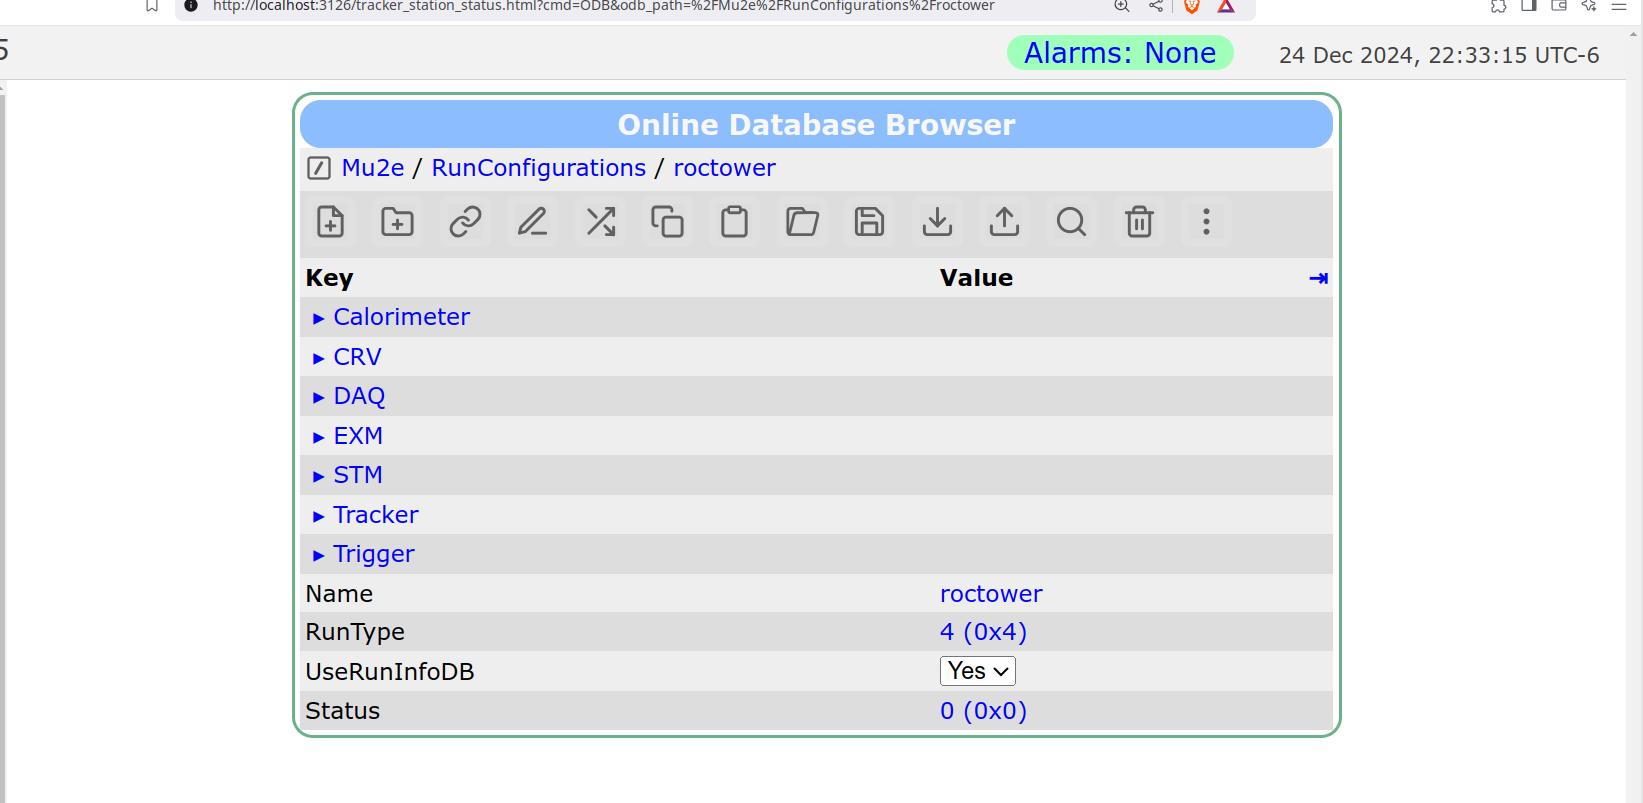
\includegraphics[width=0.95\textwidth]{png/configuration_top}
      }
    };
    % \node [text width=8cm, scale=1.0] at (14.5,0.5) {$\mu_B$, expected background mean};
    % \node [text width=8cm, scale=1.0, rotate={90}] at (1.5,7.5) { $S_{D}$, ``discovery'' signal strength  };
  \end{tikzpicture}
  \caption{
    \label{figure:configuration_top}
    Top view of the configuration called 'roctower' - a 6-ROC tracker test stand in IERC
  }
\end{figure}

%%%%%%%%%%%%%%%%%%%%%%%%%%%%%%%%%%%%%%%%%%%%%%%%%%%%%%%%%%%%%%%%%%%%%%%%%%%%%%
\subsection{Subdetector configuration}

A subdetector configuration is described by a hierarchy of elements.
Elements (substructures) are subdetector-specific, however element has
two mandatory fields: "enabled" and "status", used for configuration,
monitoring, and error reporting. A top view of the tracker configuration
is shown in Figure~\ref{figure:tracker_config}.
\begin{itemize}
\item
  enabled = 0: the element (subtree) is considered present, but not used.
\item
  enabled = 1:
  \begin{itemize}
  \item
    status = 0 : the subsystem is OK
  \item
    status < 0 : the subsystem has a problem and an action is required
    The value of the status variable is the error code
  \item
    status > 0 : the subsystem has a warning-level problem, no immediate action
    is required
  \end{itemize}
\end{itemize}

\begin{figure}[H]
  \begin{tikzpicture}
    \node[anchor=south west,inner sep=0] at (0,0.) {
      % \node[shift={(0 cm,0.cm)},inner sep=0,rotate={90}] at (0,0) {}
      \makebox[\textwidth][c] {
        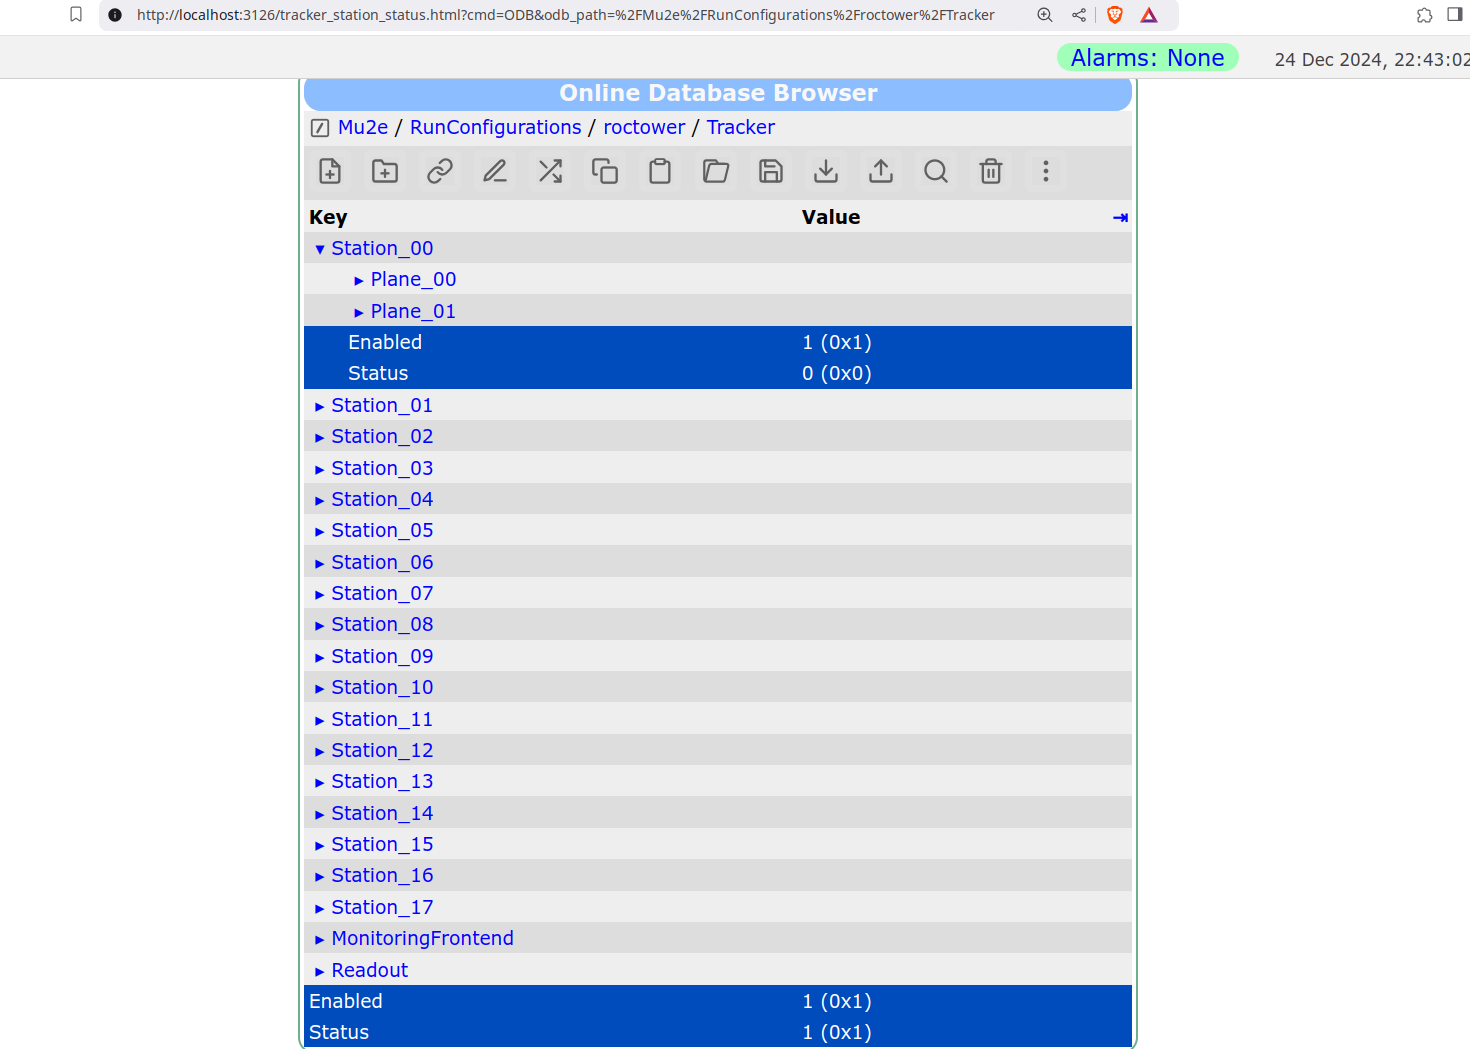
\includegraphics[width=0.95\textwidth]{png/tracker_config}
      }
    };
    % \node [text width=8cm, scale=1.0] at (14.5,0.5) {$\mu_B$, expected background mean};
    % \node [text width=8cm, scale=1.0, rotate={90}] at (1.5,7.5) { $S_{D}$, ``discovery'' signal strength  };
  \end{tikzpicture}
  \caption{
    \label{figure:tracker_config}
    Tracker configuration. The tracker, as well as each of the stations, has ``Enabled'' and
    ``Status'' fields.
  }
\end{figure}



\subsection{Data Model}

* configuration  : first step                                                
- request run number
- set "CONFIGURE" in /Mu2e/Commands/ (this could be done via the Sequencer)

- a configuration frontend (python)
  - identifies enabled subdetectors
  - passses the command to the enabled subdetector configuration frontends (python)
  - the subsystem configuration frontends are completely independent
  - waits for some time for them to act
  - subssytem configuration frontends complete, set Status and 
  - after the configuration succeeds or the time expires, the configuration
    frontend forces stop of its execution
  - it sets the command execution status and returns to MIDAS

- if the configuration step has completed successfully, a new run is started

- each subsystem has Enabled and Status attributed in ODB
- to exclude the failed sysbystem from the configuration: set Enabled=0

- DAQ configuration:

  - CFO configuration
  - configuration of each node

  - per node:

    - one or two boardreaders
    - event builder
    - data logger
    - dispatcher

    - each of them has Enabled attribute

  - TFM talks to ODB , identifies enabled processes and submits jobs only
    for them

  - there is a "Generate FCL" command which generates FCLs
    for an given? active? configuration

- as the DAQ configuration depends on the enabled detector configuration,
  the DAQ is configured afer all subdetectors 


* monitoring of the detector status                                          

- each subdetector has "Enabled" and "Status" parameters
\begin{verbatim}
|--------+-----------+--------------------------------------------|
| status | color     | meaning                                    |
|--------+-----------+--------------------------------------------|
|     -2 | dark gray | Enabled=0                                  |
|     -1 | gray      | enabled=1, but no initialization performed |
|      0 | red       | enabled=1, failed initialization           |
|      1 | green     | enabled=1, initialized OK                  |
|--------+-----------+--------------------------------------------|
\end{verbatim}

* description in ODB                                                         
- no links across configuration boundaries
- links allowed within the configuration , i.e.
  - DTC --> tracker panel
  - boardreader DTC --> DTC configuration
- ActiveConfiguration
* commands and execution
 a command has three fields
 
1) Run     : 0: "no request to run"  1: "requested to run" 
2) Status  : int
   < 0: "execution failed" , the value gives the error code
   0  : "execution finished OK"
   1  : "execution in progress"

   after the Status is set, the same client resets Run=0
3) Parameters :


%%%%%%%%%%%%%%%%%%%%%%%%%%%%%%%%%%%%%%%%%%%%%%%%%%%%%%%%%%%%%%%%%%%%%%%%%%%%%%
\subsection{Configuration of the frontends}

\begin{itemize}
\item
  one monitoring/control frontend per DAQ server . MOnitoring:
  \begin{itemize}
  \item
    2 DTC's with 6 ROCs per DTC
  \item
    ARTDAQ processes:
    \begin{itemize}
    \item
      2 boardreaders, N event builders, potentially a data logger, and a dispatcher
    \end{itemize}
  \item
    overall health: amount of free space available
  \end{itemize}
\item
  global control frontend:
\end{itemize}
%%% Local Variables:
%%% mode: latex
%%% TeX-master: t
%%% End:

\section{Interface to ARTDAQ}

ARTDAQ processes are controlled by the special MIDAS ``
Trigger Farm Manager (TFM) frontend'', tfm\_launch\_fe.py.

The TFM frontend runs the TFM manager which inherits the functionality
of artdaq\_daqinterface, providing an interface between the MIDAS-based
run control system and ARTDAQ.

The TFM reads its initial settings from ODB. its configuration path is "/Mu2e/ActiveRunConfiguration/DAQ/Tfm"


%%% Local Variables:
%%% mode: latex
%%% TeX-master: t
%%% End:



%%%%%%%%%%%%%%%%%%%%%%%%%%%%%%%%%%%%%%%%%%%%%%%%%%%%%%%%%%%%%%%%%%%%%%%%%%%%%%
\section{Run-time diagnostics and error reporting}

At run-time, the status of the system is visualized by the system status tree.
The top page of the tree is shown in Figure~\ref{figure:mu2e_status_page}.

\begin{itemize}
\item
  one monitoring frontend per DAQ node, monitors the DTCs and the ARTDAQ processes.
  The frontend is responsible for setting status of the ROCs, boardreaders, and such.
  THe same frontend propagates the error status up the subdetector tree. 
  \item
  monitoring GUI - displays status of the detector. MIDAS-based javascript+HTML.
  Each element of the detector system, as described in ODB, in addition to other parameters
  has two mandatory ones: ``Enabled'' and ``Status''.
  \begin{itemize}
  \item 
    Setting Enabled=0 excludes the element from the configuration, in which case it will be
    shown in gray.
  \item
    Enabled=1 will result in the element shown in green (Status >= 0) or red (Status< 0) 
  \end{itemize}
\end{itemize}

\begin{figure}[H]
  \begin{tikzpicture}
    \node[anchor=south west,inner sep=0] at (0,0.) {
      % \node[shift={(0 cm,0.cm)},inner sep=0,rotate={90}] at (0,0) {}
      \makebox[\textwidth][c] {
        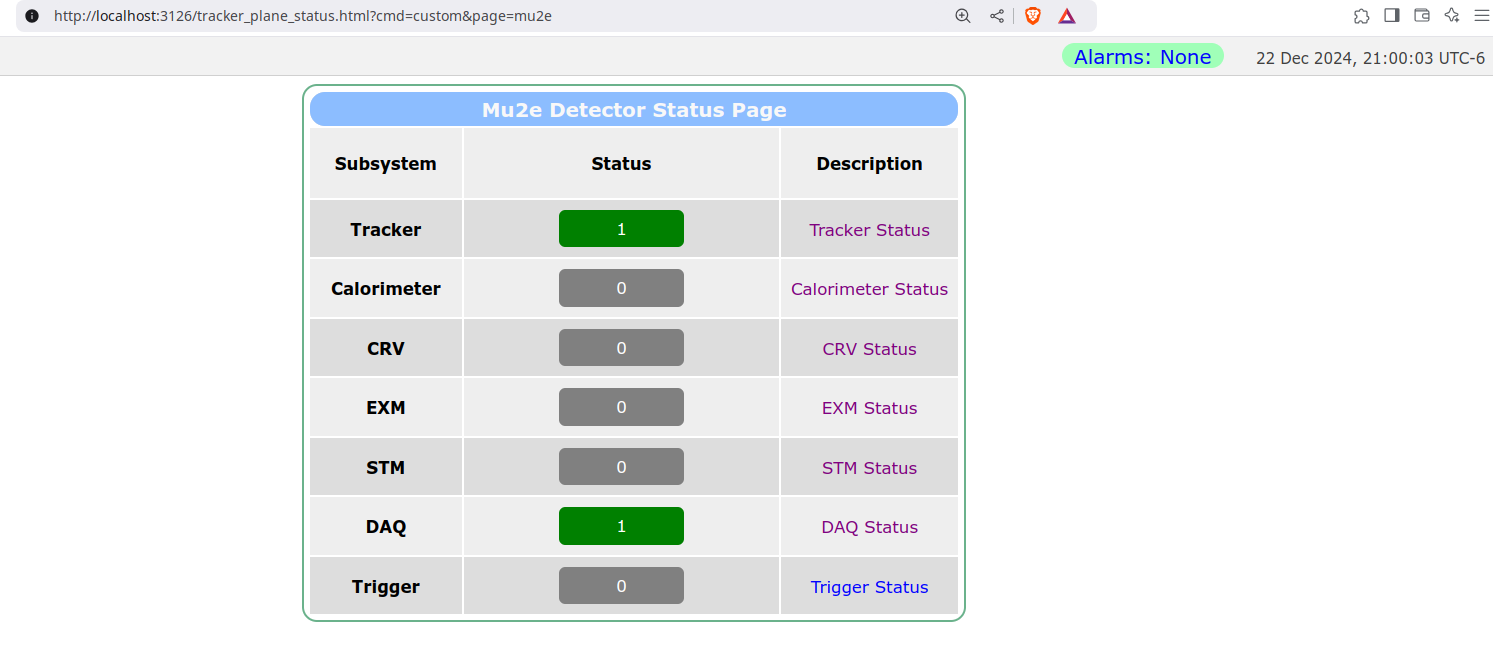
\includegraphics[width=0.95\textwidth]{png/mu2e_status_page}
      }
    };
    % \node [text width=8cm, scale=1.0] at (14.5,0.5) {$\mu_B$, expected background mean};
    % \node [text width=8cm, scale=1.0, rotate={90}] at (1.5,7.5) { $S_{D}$, ``discovery'' signal strength  };
  \end{tikzpicture}
  \caption{
    \label{figure:mu2e_status_page}
    Mu2e status page (prototype)
  }
\end{figure}

State of each enabled configurable element is monitored by a MIDAS frontend.
If a problem is detected, the status of the element is set to a negative
number, which value represents the status code of the problem.

A special configuration frontend propagates the status of the problem up the
configuration tree in ODB. For example, if a problem is detected with one of the
tracker panels, the status box corresponding to the tracker on the top monitoring
page will also become red.

After a problem with the panel is cleared, its status gets set to zero by the
monitoring frontend. The change is propagated up the configuration tree
by the configuration frontend, and the color of the tracker monitoring box
becomes green again.


THe element status box becomes red. 

%%% Local Variables:
%%% mode: latex
%%% TeX-master: t
%%% End:

%%%%%%%%%%%%%%%%%%%%%%%%%%%%%%%%%%%%%%%%%%%%%%%%%%%%%%%%%%%%%%%%%%%%%%%%%%%%%%
\section{Starting and stopping a run: operational procedures }

\begin{itemize}
\item
  request the next run number from the Mu2e run conditions database
  (MIDAS sequencer ==> config/scripts/get\_next\_run\_number.py) and store
  it in ODB (rn-1)
\item
  configure the detector using the sequencer scripts.
  When the system will become stable enough, the configuration functionality
  could be moved to the frontends.
\item
  start the run. At this point the detector is configured and ready to be read out.
  The TFM frontend starts the ARTDAQ processes , after which the CFO frontend 
  initiates new run plan.
\item
  to stop the run, the CFO frontend terminates execution of the run plan
  by the CFO, after that the TFM frontend ends the run and the TFM terminates
  the ARTDAQ processes.
\end{itemize}

%%% Local Variables:
%%% mode: latex
%%% TeX-master: t
%%% End:

%%%%%%%%%%%%%%%%%%%%%%%%%%%%%%%%%%%%%%%%%%%%%%%%%%%%%%%%%%%%%%%%%%%%%%%%%%%%%%
\section{Documentation and support considerations}

\begin{itemize}
\item
  MIDAS wiki \cite{2025_MIDAS_WIKI}, hosted by TRIUMF, serves the role of 
  of the user/developer manuals which is always up to date.
\item 
  The MIDAS forum provides an efficient way for communicating with the experts.
\item
  MIDAS is supported on Windows, Macs and Linux.
  Expect active support to continue over the lifetime of Mu2e.
\item 
  MIDAS codebase is public and maintained at: https://bitbucket.org/tmidas/workspace/projects/PROJ
\item
  significant developer base: about 4-5 core developers from several running experiments
\item
  activity over the last 12 months: 100's of commits by the core developers/maintainers plus
  13 pull requests by 6 developers
\end{itemize}




%%% Local Variables:
%%% mode: latex
%%% TeX-master: t
%%% End:


%%%%%%%%%%%%%%%%%%%%%%%%%%%%%%%%%%%%%%%%%%%%%%%%%%%%%%%%%%%%%%%%%%%%%%%%%%%%%% 
\section {Summary}



%%%%%%%%%%%%%%%%%%%%%%%%%%%%%%%%%%%%%%%%%%%%%%%%%%%%%%%%%%%%%%%%%%%%%%%%%%%%%%
%
%%%%%%%%%%%%%%%%%%%%%%%%%%%%%%%%%%%%%%%%%%%%%%%%%%%%%%%%%%%%%%%%%%%%%%%%%%%%%%
\newpage
\bibliographystyle{unsrtnat}
\bibliography{clfv,mu2e_internal_notes,mu2e_piplusenu_notes,mu2e_publications,radiative_pion_capture}

% \include{appendix_a}
\include{appendix_b}

\end{document}
